\documentclass[10pt, compress]{beamer}

\usetheme{m}

\usepackage{booktabs}
\usepackage{minted}
\usepackage{graphicx}
\graphicspath{ {images/} }

\usepgfplotslibrary{dateplot}

\usemintedstyle{trac}

\title{Environnements de MOOC avec Docker}
\subtitle{Projet de fin d'études - VAP ASR}
\date{28 Janvier 2015}
\author{François Monniot \& Alexis Mousset\\ Encadrants : Olivier Berger \& Christian Bac}
\institute{
\includegraphics[width=1cm]{logo.jpg}}
\titlegraphic{
   \includegraphics[width=2cm]{logo_TSP.jpg}
}

\begin{document}

\maketitle

\section{Introduction}

\begin{frame}[fragile]
  \frametitle{MOOC}

  Un MOOC est un \emph{Massive Open Online Course} :
  \pause
  \begin{itemize}[<+- | alert@+>]
  \item Adapté à de nombreux utilisateurs
  \item Ouvert à tous
  \item Communication par Internet
  \item Participants éloignés géographiquement
  \end{itemize}

\end{frame}

\begin{frame}[fragile]
  \frametitle{Contexte}

  \begin{itemize}[<+- | alert@+>]
  \item MOOC lancé à Télécom SudParis en 2013 (sur Moodle)
  \item Plusieurs projets à l'école et dans l'institut, ou Paris-Saclay
  \item Environnement de TP pour les bases de données basé sur Vagrant
  \item Besoin de continuer à créer des environnements de TP
  \end{itemize}
\end{frame}

\begin{frame}[fragile]
  \frametitle{Proposition Docker}

\end{frame}

\section{Docker}

\begin{frame}[fragile]
  \frametitle{Qu'est-ce qu'un conteneur ?}
  \begin{center}
  % lxc commence en 2008
  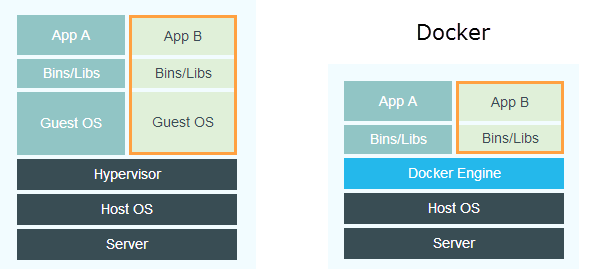
\includegraphics[scale = 0.5]{dockervsvm.png}
   \end{center}
\end{frame}

\begin{frame}[fragile]
  \frametitle{Develop, Ship and Run Any Application, Anywhere}
  Qu'apporte Docker ?
  \pause
  \begin{itemize}[<+- | alert@+>]
  \item Workflow intégrant tout le cycle du vie de l'application
  \item Rapide à créer, déployer et exécuter
  \end{itemize}
  \pause
   Comment ?
   \pause
  
\begin{itemize}[<+- | alert@+>]
  \item Docker Engine (démon + client)
    \begin{itemize}[<+- | alert@+>]
      \item Conteneurs jetables
      \item Images : layers, AUFS, versionning
      \item Volumes
      \item Liens
    \end{itemize}
  \item Docker Hub
  \begin{itemize}[<+- | alert@+>]
      \item Contient des images
      \item Images officielles
      \item Images publiques
      \item Images privées
    \end{itemize}

\end{itemize}
\end{frame}

\section{Implémentation}

\begin{frame}[fragile]
  \frametitle{Outils utilisés}

  \begin{itemize}
      \item Docker
      \item Fig
      \item Mosquitto
      \item PHP
      \item Moodle
      \item Python
      \item Flask
    \end{itemize}
  
\end{frame}

\begin{frame}[fragile]
  \frametitle{Remontée des événements}
  \begin{center}
  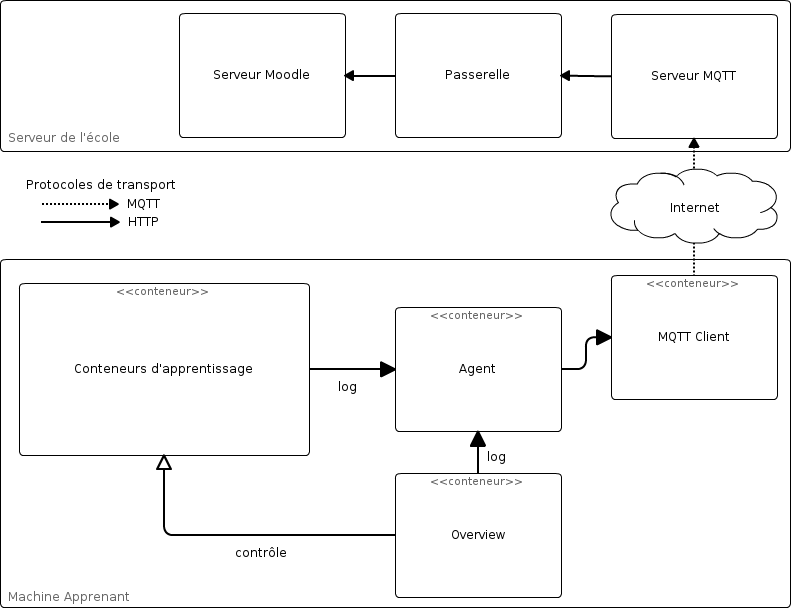
\includegraphics[scale = 0.32]{architecture.png}
   \end{center}
\end{frame}

\begin{frame}[fragile]
  \frametitle{Plugin moodle}
  \begin{center}

   \end{center}
\end{frame}

\begin{frame}[fragile]
  \frametitle{Reporting}
  Architecture :
   \begin{center}
  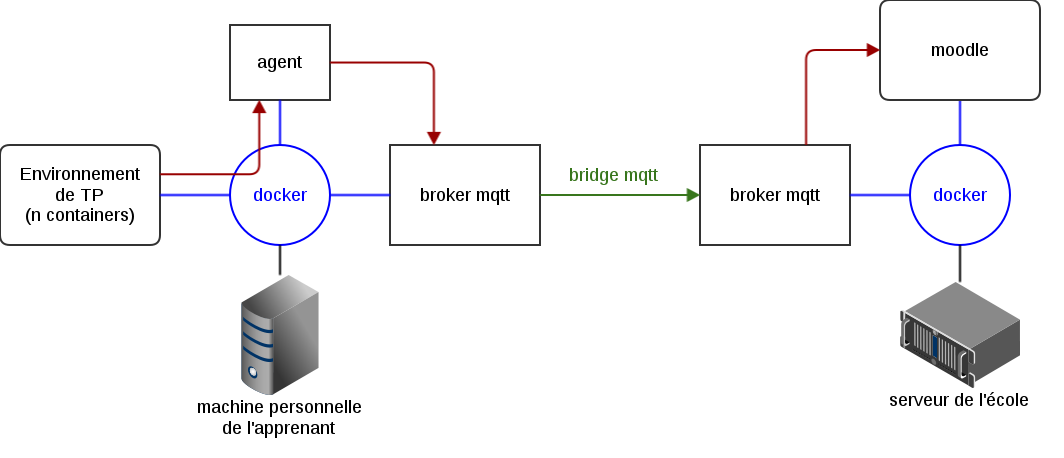
\includegraphics[scale = 0.3]{reporting.png}
   \end{center}
\end{frame}

\begin{frame}[fragile]
  \frametitle{Reporting}
  Architecture :
   \begin{itemize}[<+- | alert@+>]
      \item Bibliothèque Docker en Python
      \item Partage du socket de contrôle du démon
      \item Filtrage des logs intéressants
    \end{itemize}
\end{frame}

\begin{frame}[fragile]
  \frametitle{Tracker}
  \begin{center}

   \end{center}
\end{frame}

\begin{frame}[fragile]
  \frametitle{Overview}
  \begin{center}

   \end{center}
\end{frame}

\section{Utilisation}

\begin{frame}[fragile]
  \frametitle{Création des conteneurs}
  \begin{center}
  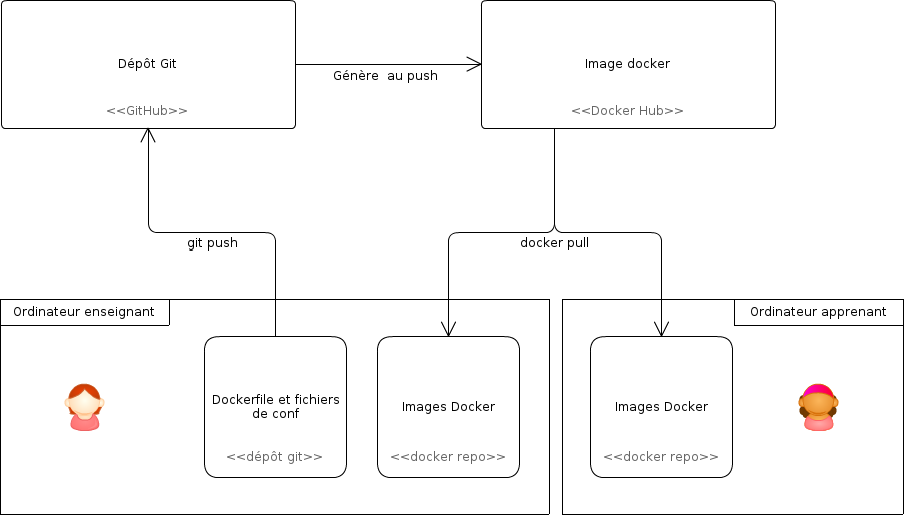
\includegraphics[scale = 0.35]{infrastructure-creation.png}
   \end{center}
\end{frame}

\begin{frame}[fragile]
  \frametitle{Enseignant}

  Exemple de \emph{Dockerfile} :

  \begin{minted}[fontsize=\footnotesize]{bash}
FROM postgres:9.3
# scripts de peuplement des bases de données
COPY ./db-creation /db-creation
# script exécuté à la création de l'instance
RUN mkdir -p /docker-entrypoint-initdb.d
COPY ./initdb-setupdb.sh /docker-entrypoint-initdb.d/setupdb.sh
  \end{minted}
  
  Lancement d'une instance basée sur cette image :
  
  \begin{minted}[fontsize=\footnotesize]{bash}
docker build -t mydb .
docker run mydb
  \end{minted}
\end{frame}

  \begin{frame}[fragile]
  \frametitle{Fig}

  Exemple de configuration \emph{fig.yml} :

  \begin{minted}[fontsize=\footnotesize]{bash}
web:
  build: web
  links:
   - db
  ports:
   - "8000:8000"
db:
  image: postgres
  \end{minted}
  
  Création et lancement des conteneurs :
  
    \begin{minted}[fontsize=\footnotesize]{bash}
fig up
  \end{minted}
\end{frame}

\begin{frame}[fragile]
  \frametitle{Apprenant}

  \begin{itemize}[<+- | alert@+>]
      \item Installation de boot2docker (ou docker si sous Linux)
      \item Lancement de boot2docker
      \item Configuration des accès Moodle dans un fichier
      \item Exécution de scripts d'installation : téléchargement des images, lancement des conteneurs
      \item Lancement d'une éventuelle interface web dans le navigateur, en local
    \end{itemize}
\end{frame}


\section{Démonstration}

\plain{Questions ?}

\end{document}
